%\documentclass[h, xcolor=pst, dvips]{beamer} % presentation normale avec du PSTricks (dvi->ps->pdf)

\documentclass{beamer}

\mode<article> % pour la version 'article'
{
  \usepackage{fullpage}
  \usepackage{hyperref}
}


\mode<presentation> % pour la version 'presentation'
{
  \usetheme{Warsaw} % Warsaw Frankfurt
}


\usepackage[frenchb]{babel}     % specification francaise
\usepackage[latin1]{inputenc}   % entree clavier latin1
% \usepackage[T1]{fontenc}        % sortie

% \usepackage{nameref} % permet d'�crire le nom de la section en cours
% (n�cessite 2 compilations)

\usepackage{graphicx}
\usepackage{tabularx}

\renewcommand{\emph}[1]{\textcolor{red}{\underline{\textit{\textcolor{black}{#1}}}}}

%\newcommand{\inclure}[1]{
%  \graphicspath{%
%    {#1/}%
%  }
%  \tp{D�termination par conductim�trie\\
de la concentration en solut�\\
d'une solution ionique}


\begin{multicols}{2}

\objectifs{
\item r�aliser une courbe d'�talonnage $G = f(C)$ et en d�duire une
  concentration inconnue.
\item Aborder une limite de la m�thode d'�talonnage.
}
\vspace*{2cm}


\materiel{
\item b�cher $600~mL$
\item fiole jaug�e $500~mL$
\item burette gradu�e $25~mL$
\item pipette jaug�e $5~mL$
\item agitateur magn�tique.
\item solution de chlorure de sodium $S_0$ de concentration $C_0 =
  0,10~mol.L^{-1}$
\item flacon de s�rum physiologique
\item eau d�min�ralis�e
\item g�n�rateur basse fr�quence.
\item 2 multim�tres
\item cellule de conductim�trie.
}


\end{multicols}




\section{R�alisation d'une �chelle de conductance}


\begin{multicols}{2}

\subsection{Protocole op�ratoire}
\begin{enumerate}
\item Rincer la burette, la remplir � l'aide de la solution $S_0$ ajuster le
z�ro.

\item Avec la fiole jaug�e, introduire $V = 500~mL$ d'eau d�min�ralis�e dans
le b�cher.

\item Placer la cellule conductim�trique dans le b�cher et r�aliser le
montage �lectrique correspondant au sch�ma ci-contre. Les 2
multim�tres sont en mode alternatif ($AC$ ou \acsymbol).

\item Sur le GBF, r�gler la fr�quence $500~Hz$ et fixer la tension �
$1,00~V$.

\item Au contenu du b�cher, ajouter les volumes $V_0$ suivants de solution
de chlorure de sodium mesur�s pr�cis�ment gr�ce � la burette. Apr�s
chaque addition, v�rifier que la tension est toujours de $1,00~V$ et
relever la valeur de l'intensit�.

\end{enumerate}




\begin{center}
\begin{figure}[H]
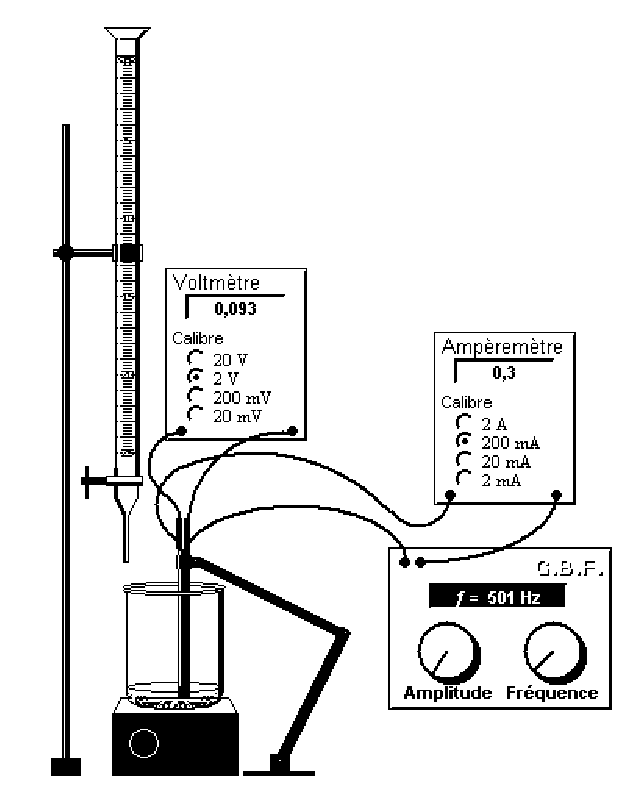
\includegraphics[width=6cm]{tp_prem_s_chimie/tp6_determination_par_conductimetrie_concentration/montage_conductimetrie.png.eps}
\caption{Dispositif exp�rimental}
\end{figure}
\end{center}


\end{multicols}



\subsection{R�sultats}
\begin{enumerate}
\item Calculer la conductance $G$ et compl�ter le tableau suivant.

\begin{arraydata}{6}
\hline
$V_0$ ($mL$)       &  0 &  5 & 10 & 15 & 20 & 25 \\ \hline
\rule[-0.4cm]{0cm}{1cm}
$C$ ($mol.L^{-1}$) &    &    &    &    &    &    \\ \hline
\rule[-0.4cm]{0cm}{1cm}
$G$ ($mS$)         &    &    &    &    &    &    \\ \hline
\end{arraydata}

\item Tracer la courbe d'�talonnage $G = f (C)$.
\end{enumerate}



\pagebreak
%\newpage


\section{D�termination de la concentration en $NaCl$ d'une solution de
  s�rum physiologique}

L'objectif est de d�terminer la concentration du chlorure de sodium dans le s�rum physiologique injectable.

\begin{enumerate}
\item Diluer au $1/100\ieme$ le s�rum physiologique. En pr�parer $500~mL$.

\item D�crire � l'aide de sch�mas le protocole utilis� pour r�aliser
  cette dilution au $1/100\ieme$ et obtenir la solution $S'$.

\item D�terminer la conductance $G'$ de cette solution $S'$.

\item En d�duire la concentration $C'$ du chlorure de sodium dans le
  s�rum physiologique dilu�.

\end{enumerate}


\vressort{3}

\section{Questions compl�mentaires}

%\begin{multicols}{2}

\begin{enumerate}
\item Expliquer comment calculer la concentration $C$ des diff�rentes
  solutions de chlorure de sodium. Donner l'expression de $C$ en
  fonction de $C_0$, $V_0$, $V$.


\item Comment calcule-t-on la conductance $G$ ?

\item Pour quelle raison pratique a-t-on int�r�t � prendre $U =
  1,00~V$ dans les diff�rentes manipulations ?

\item En extrapolant la courbe d'�talonnage, pr�voir la conductance
  d'une portion de solution concentr�e � $T = 58,4~g.L^{-1}$. Mesurer
  la conductance r�elle d'une portion d'une telle solution. Que
  peut-on conclure quant � la m�thode d'�talonnage utilis�e. On donne
  $M_{Na} = 23~g.mol^{-1}$ et $M_{Cl} = 35,5~g.mol^{-1}$.

\item Rappeler la valeur de la concentration $C'$ du chlorure de
  sodium dans le s�rum physiologique dilu�.

\item Comment peut-on alors d�terminer la concentration $C_0'$ du
  chlorure de sodium dans la solution commerciale de s�rum
  physiologique ? Calculer cette concentration $C_0'$ puis le titre
  massique (concentration massique) correspondant $T_0$. Le comparer avec
  les indications figurant sur l'�tiquette du flacon ($0,9~\%$ en masse).
\end{enumerate}


%\vressort{1}
\vressort{3}

\begin{center}
\begin{figure}[H]
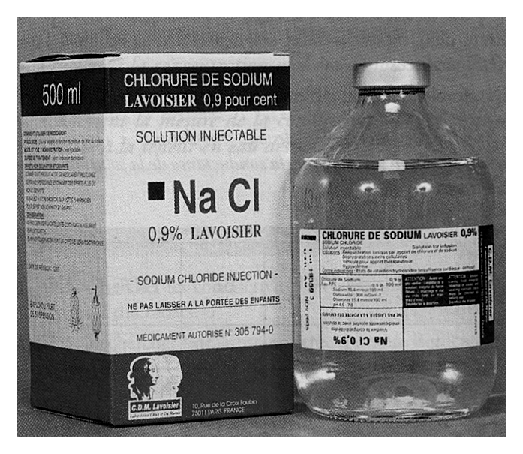
\includegraphics[width=7cm]{tp_prem_s_chimie/tp6_determination_par_conductimetrie_concentration/solution_nacl.png.eps}
\caption{Solution de chlorure de sodium}
\end{figure}
\end{center}


%\end{multicols}


\vressort{3}
%}

\graphicspath{%
  {../frames/}%
}

% PSTricks
% \usepackage{pstricks}
% \usepackage{pst-plot} % trac� de fonctions
% \usepackage{pst-circ} % circuit en elec

\newcommand{\actuellement}[1]{%
  \textit{#1}
  % \emph{#1}
}

\newcommand{\vressort}[1]{%
  \vspace{\stretch{#1}}
}

%\inclure{poste}
\newcommand{\poste}{%
  Poste 1477\\
  PRAG\\
  \'Ecole Nationale Sup�rieure de Chimie Lille\\
}

\newcommand{\presposte}{%
\section{Pr�sentation du poste}

\frame{
  \frametitle{\insertsectionhead}
  % \pause


  \begin{tabularx}{\linewidth}{XX} %{p{13cm}X}

    \begin{center} % flushright
      \poste
    \end{center}

    &

    \vspace*{\stretch{1}}

    \begin{center}
%      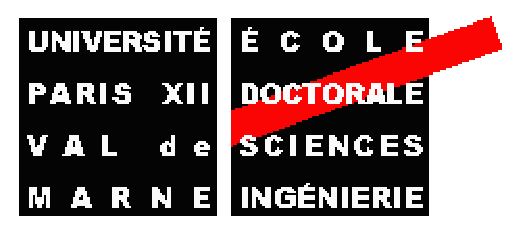
\includegraphics[width=3cm]{logo.gif} % avec pdflatex
      
\includegraphics[width=3cm]{logo.eps} % avec latex
    \end{center}

    \vspace*{\stretch{1}}

  \end{tabularx}


%  \begin{itemize}
%  \item Polytech'Grenoble
%  \end{itemize}
}
}

\newcommand{\conclusion}{%
\section{Conclusion}
\frame{
  \frametitle{\insertsectionhead}

  \vspace{\stretch{5}}

  \begin{center}
    \begin{Huge}
      En conclusion...
    \end{Huge}
  \end{center}
  

  \vspace{\stretch{5}}
}
}

\date{Mercredi 24 Janvier 2007} % poste

\title{\poste}
%\title{Titre}

\author{S�bastien \textsc{CELLES}}

\institute{Professeur agr�g� de Sciences Physiques - Physique Appliqu�e}

% \date{\today}
% \subject{...}

\begin{document}

\frame{
  % \maketitle
  \titlepage
}


\frame
{
  \tableofcontents
}


\presposte % presentation poste

%\frame{
%  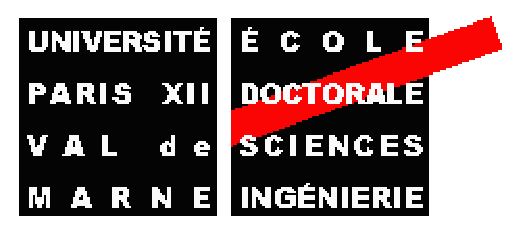
\includegraphics[width=3cm]{logo.gif.eps}
%}

% parcours scolaire
\section{Parcours scolaire et universitaire}

\frame{
  \frametitle{\insertsectionhead}
  % \pause
  \begin{itemize}
  \item S�bastien \textsc{CELLES}
    % \pause
  \item Professeur agr�g� de Sciences Physiques - Physique Appliqu�e
    % \pause
    % \pause
  \item N� � Brive (Corr�ze) le 3 Juillet 1978
    % \pause
  \item \'Etudes secondaires g�n�rales (fili�re Scientifique)
    % \pause
  \item \'Etudes sup�rieures
    % \pause
    \begin{itemize}
    \item Classes Pr�paratoires aux Grandes Ecoles (PCSI, PSI)
      % \pause
    \item Universit�
      % \pause
      \begin{itemize}
      \item Licence de Physique
        % \pause
      \item Ma�trise EEA (\'Electronique, \'Electrotechnique, Automatique)
      \end{itemize}        
    \end{itemize}
    % \pause
  \item CAPES de Physique Appliqu�e en 2001
    % \pause
  \item Agr�gation de Physique Appliqu�e en 2003
  \end{itemize}
}



% enseignement
\section{Parcours au sein de l'\'Education Nationale}

\frame{
  \frametitle{Mon parcours au sein de l'\'Education Nationale}

  % \pause

  \begin{itemize}
  \item Professeur stagiaire (2002-2003)
    \begin{itemize}
    \item Physique Chimie en 5$^{\mbox{i\`eme}}$,
      4$^{\mbox{i\`eme}}$\\
      (Coll�ge Jules Vernes - DEVILLE-LES-ROUEN)\\
      Stage en situation

      % \pause

    \item Physique Appliqu�e en 1$^{\mbox{i\`ere}}$ et Terminale \'Electronique\\
      (Lyc�e Marcel SEMBAT - SOTTEVILLE-LES-ROUEN)\\
      Stage de pratique accompagn�e
    
    \end{itemize}
  \end{itemize}
}

\frame{
  \frametitle{Mon parcours au sein de l'\'Education Nationale (suite)}
  

  \begin{itemize}
  \item Titulaire en Zone de Remplacement (TZR) dans le
    d�partement de la Haute-Vienne (depuis 2003)
    \begin{itemize}

    \item Classes Pr�paratoires aux Grandes \'Ecoles\\
      \small (Math. Sup. PCSI - Lyc�e Gay Lussac - LIMOGES)
      
      % \pause

      \normalsize

    \item Physique Industrielle en BTS CIRA\\
      \small (Lyc�e Raoul DAUTRY - LIMOGES)
      
      % \pause

      \normalsize
    \item Physique Appliqu�e en lyc�e technologique\\
      1$^{\mbox{i\`ere}}$ \'Electrotechnique,
      Terminale G�nie M�canique\\ \small
      (Lyc�e TURGOT - LIMOGES)
      
      % \pause

      \normalsize
      
    \item Physique Chimie en lyc�e g�n�ral\\ \small
      1$^{\mbox{i\`ere}}$ Scientifique,
      1$^{\mbox{i\`ere}}$ STL C, %Sciences et Techniques de Laboratoire
      Terminale STL Biochimie,
      \actuellement{Seconde Tronc commun et option PCL}\\
      (Lyc�e Raoul DAUTRY - LIMOGES)
      
      \normalsize   
      
    \end{itemize}
  \end{itemize}
}

% formation info
% formation � distance
% crdp

\frame{
  \frametitle{Autres activit�s au sein de l'\'Education Nationale}

  \begin{itemize}
  \item Formation informatique pour les enseignants
    et les personnels de laboratoire\\
    \begin{itemize}
    \item Notions sur les r�seaux (classe de r�seau, adresse IP)
    \item Notions sur Windows (installation, s�curit�, partage...)
    \item Notions sur le web (aspirer un site, publier un site...)
    \item Quelques applications en milieu scolaire (VNC)
    \item Introduction � quelques logiciels libres
      \begin{itemize}
      \item OpenOffice.org
      \item GIMP
      \end{itemize}
    \end{itemize}
  \end{itemize}
\begin{center}
\url{http://www.celles.net/wikini/wakka.php?wiki=}\\
\url{InfoDautryFormation}
\end{center}
}
\frame{
  \frametitle{Autres activit�s au sein de l'\'Education Nationale}

  % 2006-2007 Dautry

  \begin{itemize}
  \item Syst�me de suivi des cours par internet pour une �l�ve hospitalis�e.
    
    \begin{itemize}
    \item Mise en place de SPIP
    \item Formation des �l�ves � l'utilisation en tant que r�dacteur
    \end{itemize}
  \end{itemize}
 
\begin{center}
\url{http://lyc-dautry-87.ovh.org}\\
\end{center}
}
\frame{
  \frametitle{Autres activit�s au sein de l'\'Education Nationale}
  \begin{itemize}
  \item Missions au Centre R�gional de Documentation P�dagogique (LIMOGES)
    \begin{itemize}
    \item R�alisation de maquettes et de documents
      sur les �nergies renouvelables
      \begin{itemize}
      \item \'Energie solaire thermique
      \item \'Energie solaire photovolta�que
      \item \'Energie �olienne
      \item \'Energie hydro�lectrique
      \end{itemize}
    \item R�alisation de documents pour divers mat�riels
      \begin{itemize}
      \item \'Etude des ondes sonores
      \item Mini syst�me d'EXAO
      %\item Mini GBF
      \end{itemize}
    \end{itemize}
  \end{itemize}
\begin{center}
\url{http://www.celles.net/wikini/wakka.php?wiki=}\\
\url{CRDP}
\end{center}
}

\frame{
  %\frametitle{\insertsubsectionhead}
  \frametitle{Membre de jury d'examens ou de concours}

  \begin{itemize}
    \item Baccalaur�at Sciences et Technologie Industrielle (STI) \\
      G�nie M�canique (Juin/Juillet 2005)
    \item Baccalaur�at Sciences et Technologie de Laboratoire (STL) \\
      Biochimie / G�nie Biologique (Juin/Juillet 2006)
  \end{itemize}
}

% \section{En quoi mon parcours est-il adapt� � ce poste ?}

% \frame{
%   \frametitle{\insertsectionhead}

%   \vspace{\stretch{5}}

%   \begin{center}
%     \begin{Huge}
%       En quoi mon parcours convient-il � ce poste ?
%     \end{Huge}
%   \end{center}
  

%   \vspace{\stretch{5}}
% }

% info g�n�rale

% langage C
%\subsection{Informatique g�n�rale (langage C)}

\frame{
  \frametitle{\insertsubsectionhead}

  % \pause
  
  \begin{itemize}
  \item Programmation en langage C en ma�trise EEA � l'Universit� Paul
    Sabatier - TOULOUSE III

    % \pause
    
  \item Lecture du livre langage C de \textsc{KERNIGHAN} et
    \textsc{RICHIE}
    
    % \pause
    
  \item Connaissance des outils GNU Make et des Autotools (autoconf, automake)
    
  \end{itemize}
}

% info indus (microcontroleurs)
%\subsection{Informatique industrielle (microcontr�leurs)}

\frame{
  \frametitle{\insertsubsectionhead}

  % \pause

  \begin{itemize}
  \item Programmation de microcontr�leurs SAB Siemens C167\\ en langage C
    % \pause
    \begin{itemize}
    \item D�veloppement dans un environnement GNU/Linux
      % \pause
    \item D�veloppement avec GNU Emacs
      % \pause
    \item R�alisation d'un syst�me de distribution de carburant avec
      carte magn�tique (utilisation des interruptions pour la
      lecture de la carte, utilisation des listes cha�n�es pour la
      base de clients, ...)

    \end{itemize}
    
    % \pause

  \item Lectures sur la programmation en assembleur de PIC 16F
    %(cours de \textsc{BIGONOFF})

    % \pause

  \item Programmation en langage C des
    microcontr�leurs ATMEL AVR (ATmega8 et 16) - projets Liberlab, Arduino, OpenChrono
    
    %(articles de GNU/Linux Magazine France, documentation de gcc-avr, projet OpenChrono)

    
  \end{itemize}  

}

% r�seau
%\subsection{R�seaux locaux}

\frame{
  \frametitle{\insertsubsectionhead}
  %\frametitle{R�seaux locaux}

  % \pause


  \begin{itemize}
  \item Connaissance du mod�le OSI
    
    % \pause

  \item Lecture : les r�seaux, Guy \textsc{PUJOLLE}
    
    % \pause

  \item R�alisation d'un r�seau personnel
    % \pause
    \begin{itemize}
    \item routeur/firewall sous GNU/Linux IPCop
      % \begin{itemize}
      % \end{itemize}
      % \pause
    \item serveur sous GNU/Linux Debian
      % \pause
      \begin{itemize}
      \item Secure Copy scp par SSH
      \item VNC dans tunnel SSH, export display
      \item Samba
      \item NFS
      \item ...
      \end{itemize}
      % \pause
    \item 2 postes clients
    \end{itemize}
    % \pause
  \item Pratique du routage avec les r�gles iptables sous Linux
  \end{itemize}

  
}


% serveurs
%\subsection{Serveurs (web, base de donn�es)}

\frame{
  \frametitle{\insertsubsectionhead}
  %\frametitle{Serveurs (web, base de donn�es)}

  % \pause

  \begin{itemize}
  \item Utilisation du serveur web Apache
    % \pause
  \item Langage de scripts PHP avec base de donn�es MySQL
    % \pause
  \item Administration base de donn�es MySQL avec PhpMyAdmin
  \end{itemize}
}

% telecom
%\subsection{T�l�communications}

\frame{
  \frametitle{\insertsubsectionhead}

  % \pause

  \begin{itemize}
  \item Micro-ondes (lignes, guides, propagation, param�tres S, abaque de Smith)
    % \pause
  \item Traitement du signal
    % \pause
  \item Transmission en bande de base
    % \pause
  \item Modulations analogiques (AM, BLU, FM)
    % \pause
  \item Modulations num�riques (ASK,PSK, FSK)
  \end{itemize}
}

% unix linux
%\subsection{Unix - Linux}

\frame{
  \frametitle{\insertsubsectionhead}

  % \pause

%\begin{center}
%\emph{Utilisation courante des syst�mes Unix et/ou GNU/Linux}
%\end{center}

    % \pause
    \begin{itemize}
    \item Utilisation courante des syst�mes Unix et/ou GNU/Linux
    \item Arborescence, fichiers, liens, droits,
      % \pause
    \item Processus, signaux
      % \pause
    \item Shell : GNU BASH
      % \pause
    \end{itemize}
}


% logiciels libres
%\subsection{Logiciels libres}
\frame{
  \frametitle{\insertsubsectionhead}

%  \begin{center}
%    \emph{Go�t pour les logiciels libres}
%  \end{center}

    \begin{itemize}
      
      % \pause
      
    \item Participation � certains projets libres (rapport de bugs
      essentiellement)

      % \pause
      
    \item Cela m'a permis de mieux connaitre les outils (Bugzilla,
      CVS ou Subversion) utilis�s dans ce mode de d�veloppement
    \end{itemize}
    
    % \pause
}


%\subsection{Thermodynamique, thermique, m�canique des fluides et �nergie}
% [Thermodynamique, thermique, m�canique des fluides et �nergie]
\frame{
  \frametitle{\insertsubsectionhead}
  %\frametitle{Thermodynamique, thermique, m�canique des fluides et �nergie}

  \begin{itemize}
  \item Enseignement de la thermodynamique et de la thermique
    \begin{itemize}
    \item Physique en Math�matiques Sup�rieures PCSI
    \item Physique Industrielle en BTS CIRA
    \end{itemize}
  \item Int�r�t pour..
    \begin{itemize}
    \item karting
    \item a�ronautique 
    \end{itemize}
  \end{itemize}
}

%\subsection{Informatique}
\frame{
  \frametitle{\insertsubsectionhead}

  % \begin{center}
  %   \emph{Go�t pour les logiciels libres}
  % \end{center}
  
  \begin{itemize}
  \item Connaissance du d�veloppement web : HTML, CSS, JavaScript, PHP
  \item Connaissance des outils modernes du Web (Content Management
    System comme SPIP, Wiki, Forum...)
    
    % \pause
    
  \item \'Edition scientifique et technique avec \LaTeX
    
    % \pause
    
  \item Connaissance (plus ou moins approfondie) de diff�rents
    langages : Java, C, C++, Python, Ada
  
  \item Documentation de code avec Doxygen
    
    % \pause
    
  \end{itemize}
}

%\subsection{Conception et Fabrication Assist�e par Ordinateur}

\frame{
  \frametitle{\insertsubsectionhead}
  
  \begin{itemize}
    \item Conception Assist�e par Ordinateur
      \begin{itemize}
      \item DMT
      \item SolidWorks
      \item Autocad
      \end{itemize}
    \item Fabrication Assist�e par Ordinateur
      \begin{itemize}
      \item Mat�riel
        \begin{itemize}
        \item Fraiseuse num�rique UPA Micrelec
        \end{itemize}
      \item Logiciel
        \begin{itemize}
          \item Micrelec WinUPA
%        \item Solid Concept
%          \item CamWorks
        \end{itemize}
      \end{itemize}

    \item Quelques lectures
      \begin{itemize}
        \item La CFAO avec SolidWorks - 
          Edition Delagrave\\
          Jean-Michel Baron et Jean-Marie Rabreau

        \item Guide de l'usinage - 
          Fraisage Per�age Al�sage Brochage Plasturgie Moulage Tournage\\
          Edition Delagrave\\
          G. Paquet
      \end{itemize}
  \end{itemize}
}

%\subsection{Multim�dia}

\frame{
  \frametitle{\insertsubsectionhead}

  \begin{itemize}

  \item Dessin bitmap / retouche photo
    \begin{itemize}
    \item GIMP
    \item Paint Shop Pro
    \item Photoshop
    \end{itemize}

    \vressort{1}

  \item Dessin vectoriel
    \begin{itemize}
    \item OpenOffice Draw
    \item Inkscape
    \item Corel Draw
    \end{itemize}

  \end{itemize}
}

\frame{
  \frametitle{\insertsubsectionhead}

  \begin{itemize}

  \item Image de synth�se
    \begin{itemize}
    \item POV-Ray (KPovModeler)
    \item Blender
    \end{itemize}

    \vressort{1}

  \item Montage vid�o
    \begin{itemize}
    \item Adobe Premi�re
    \end{itemize} 

  \end{itemize}
}

\frame{
  \frametitle{\insertsubsectionhead}
     
  \begin{itemize}
  
  \item Animations vectorielles
    \begin{itemize}
    \item Macrom�dia Flash
    \end{itemize}

    \vressort{1}

  \item Animations bitmap (GIF anim�s)
    \begin{itemize}
    \item GIMP avec plugin GIMP Animation Package
    \item ImageReady
    \end{itemize} 

  \end{itemize}
}
    



\subsection{Quelques r�alisations (informatique)}

\frame{
  \frametitle{\insertsubsectionhead}

  \begin{itemize}

  \item fieldEB, simulateur d'�lectrostatique et de magn�tostatique
    
  \item Harmon, recomposition de signaux � l'aide des harmoniques

  \end{itemize}
}

% conclusion
\conclusion

% \frame{
%   \frametitle{\insertsubsectionhead (suite)}

%   \begin{itemize}
%   \item Un envie de 
%   \end{itemize}

% }



\end{document}